%!TEX root = ../../super_main.tex

\section{Vision Representation}
\label{sec:vision_representation}

With the two orientation questions, and hereby the four quadrants, decided upon, we have tried to create two vision representations, see \secref{sub:vision_representations}, namely the metaphor- and the proposition representation, for all the quadrants.

\subsection{Metaphor Representation}
\label{sub:metaphor_representation}

In Essence, metaphors are used to provide ideas by looking at some principles used in solutions for problems that are similar to your own problem. These principles can help one to find inspiration for a solution to a problem. We have tried to define some metaphors for our problem, and the metaphors can be seen in \figref{fig:metaphor}.

\begin{figure}[!htbp]
	\centering
	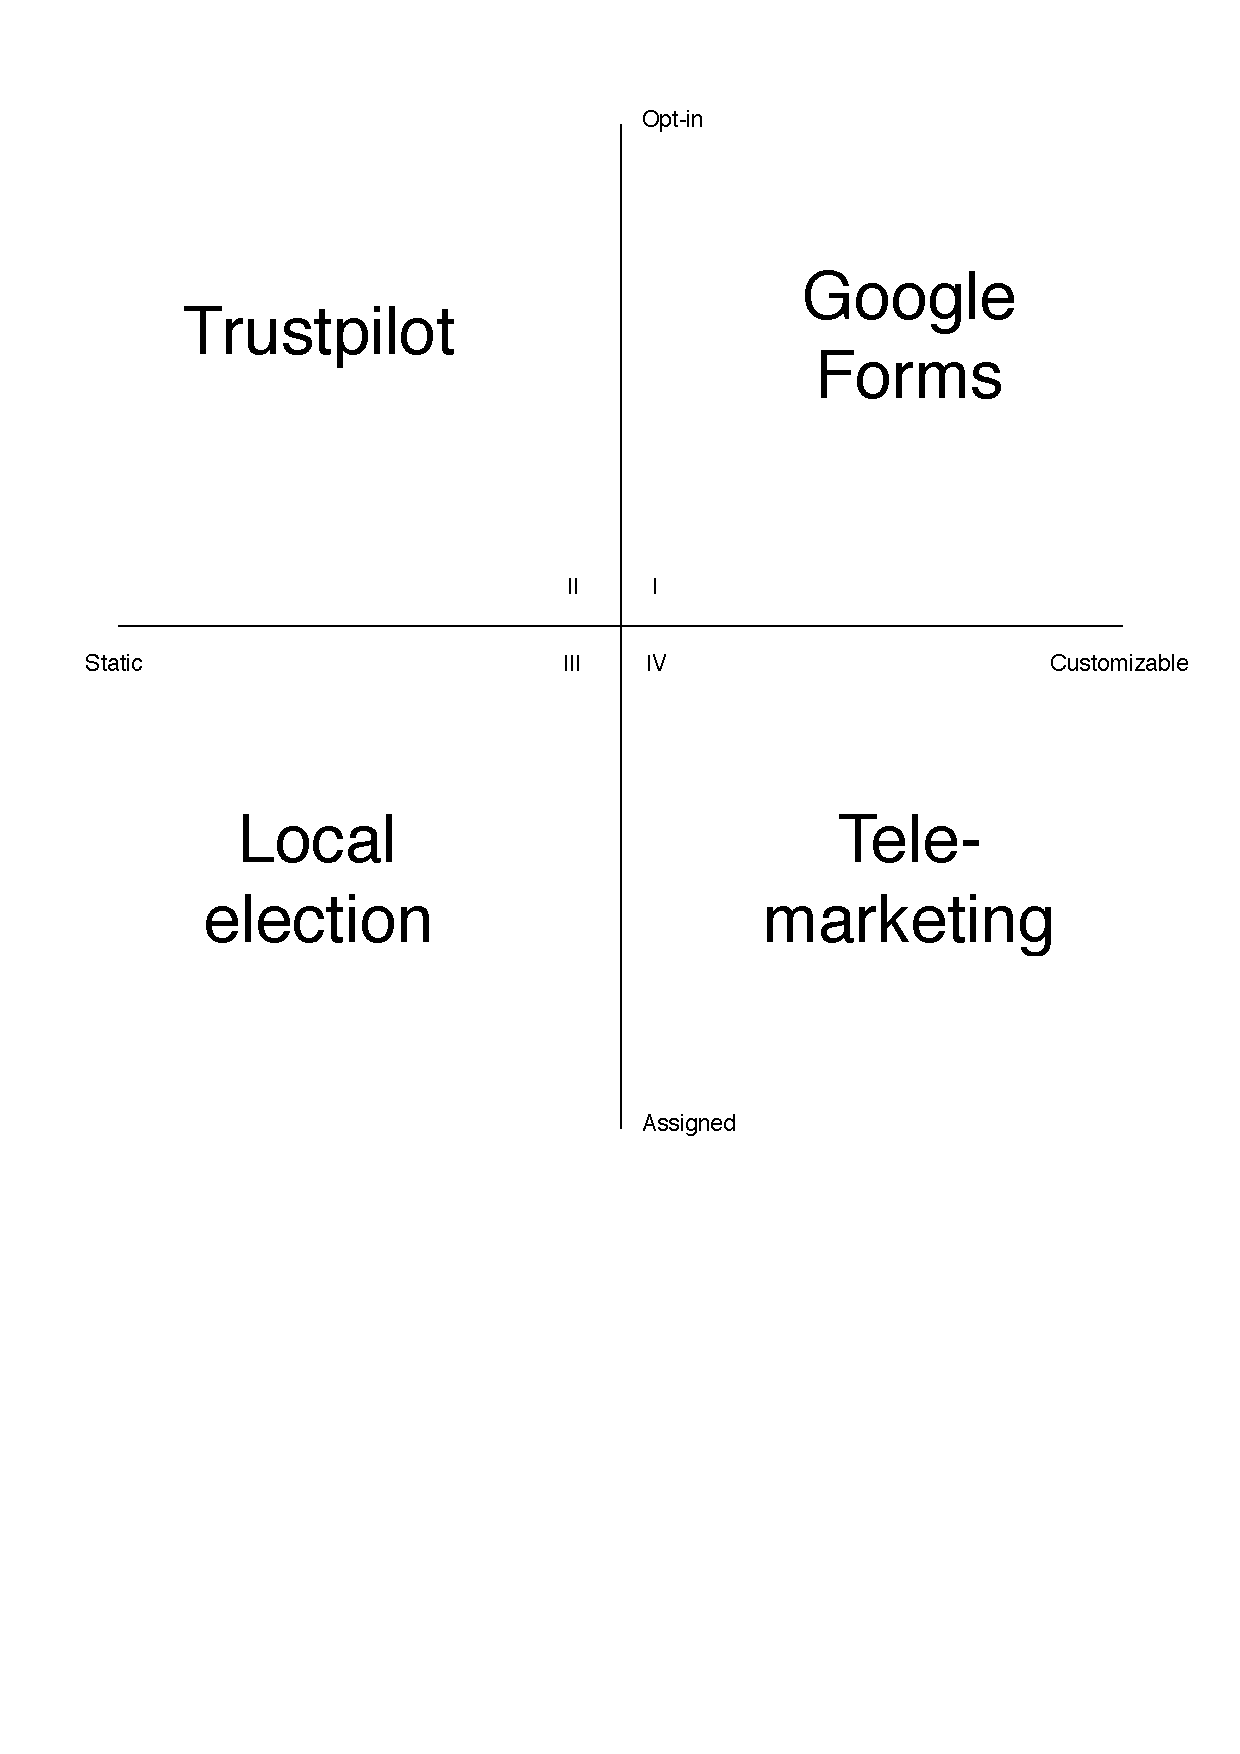
\includegraphics[width=0.8\textwidth]{graphic/problem_analysis/vision/metaphor.pdf}
	\caption{Four metaphors based upon the four quadrants.}
	\label{fig:metaphor}
\end{figure}
\FloatBarrier

The first quadrant, \emph{Google Forms}, refers to a piece of survey software, where one can create a survey and distribute it. People can then choose to either answer and not answer the questionnaire. This kind of solution can be used in our problem where participants can join a customer created campaign. The second quadrant, \emph{Trustpilot}, is a review website, where users can create reviews and rate registered online businesses. This kind of solution can be reflected in our problem, by allowing participants to opt-in on predefined campaigns. The third quadrant, \emph{Local election}, is where the inhabitants, for a specific municipality, are selected to vote at a local election. Inhabitants who do not live in the municipality, are not allowed to vote for that local election, and the voters can only vote for the listed candidates. This kind of solution can be reflected in our problem by having a profile for each of the participants, where they are assigned to campaigns that match their profile. In \emph{Telemarketing}, represented in our fourth quadrant, salespersons have profiles on potential customers. The salespersons then chooses which profiles fits best for different product they wish to sell. This kind of solution can be used in our problem, where participants fill in their profile, and the customers need to specify which kind of profiles that match their campaigns.

\subsection{Proposition Representation}
\label{sub:proposition_representation}

In Essence, a proposition is a statement or assertion that represents a design idea in a literal expression \parencite{essence_book}. Propositions can help to clarify and define scope and focus of the project. We have tried to define our design idea as propositions, where the propositions can be seen in \figref{fig:proposition}.

\begin{figure}[!htbp]
	\centering
	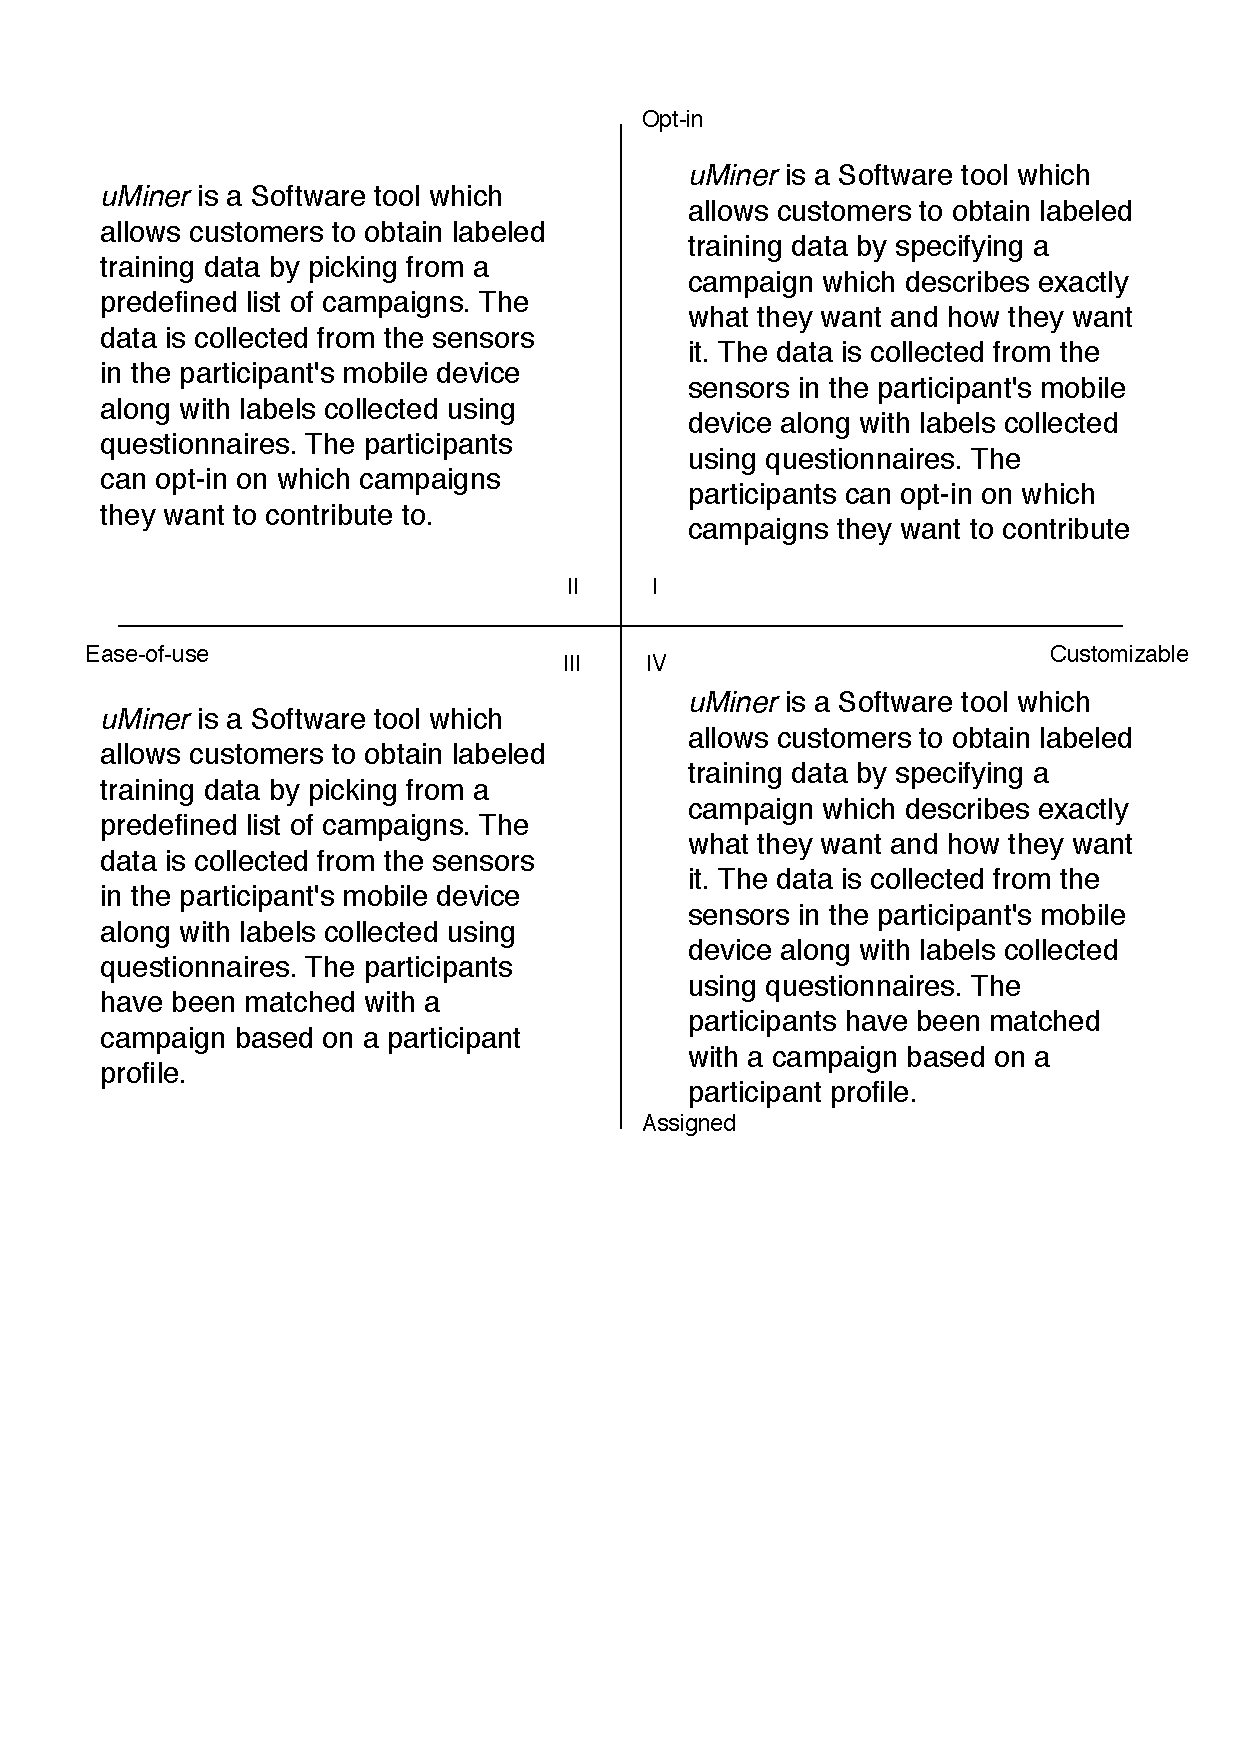
\includegraphics[width=0.8\textwidth]{graphic/problem_analysis/vision/propositions.pdf}
	\caption{Four propositions based upon the four quadrants.}
	\label{fig:proposition}
\end{figure}
\FloatBarrier

The four quadrants agree on \emph{uMiner} being a software tool that allows customers to acquire labeled training data. The data is collected using the participant's mobile device, and the system labels the data with answers from questionnaires. The quadrants vary horizontally between either having a predefined list of campaigns the customers can pick from, or that the customers can specify their own campaigns. The quadrants vary vertically between either by having the participants be able to opt-in on the campaigns they want to contribute to, or by having a profile for each participant and let their profiles to match with a campaign.
